\documentclass[12pt]{article}

\usepackage{float} 
\usepackage{amsthm}
\usepackage{hyperref}
\usepackage{marginnote}
\usepackage{bm}
\usepackage[utf8]{inputenc}
\usepackage{amsmath, amssymb}
\usepackage{titlesec}
\usepackage{graphicx} 

% Change section numbering to letters
\renewcommand{\thesection}{\Alph{section}}
\renewcommand{\thesubsection}{\thesection.\arabic{subsection}}
\renewcommand{\thesubsubsection}{\thesubsection.\arabic{subsubsection}}

% Styling sections and subsections
\titleformat{\section}{\Large\bfseries}{\thesection.}{1em}{}
\titleformat{\subsection}{\large\bfseries}{\thesubsection.}{1em}{}
\titleformat{\subsubsection}{\normalsize\bfseries}{\thesubsubsection.}{1em}{}

% Adjust spacing
\usepackage{setspace}
\setstretch{1.5}



\title{Computational Physics (PHYS414/514) \\
Final Project}
\author{Mehmet Eren Erken \\
Koç University}
\date{}

\begin{document}

\maketitle

\clearpage % Ensures the content after this starts on a new page

\section*{Newton}

This part gives calculations of the structures of various types of stars in Newtonian gravity, general relativity (GR), and alternative theories of gravity which try to surpass GR.

\section{Lane–Emden Equation}

\subsection{Stellar Structure in Newtonian Gravity}

We start with the standard Newtonian equations for hydrostatic equilibrium in a spherically symmetric star:

1. \textbf{Mass Continuity}:
   \[
   \frac{dm}{dr} = 4\pi r^2 \rho(r),
   \]

2. \textbf{Hydrostatic Equilibrium}:
   \[
   \frac{dp}{dr} = -\frac{G m(r) \rho(r)}{r^2}.
   \]

where:
\begin{itemize}
    \item \( m(r) \): mass enclosed within radius \( r \),
    \item \( \rho(r) \): mass density,
    \item \( p(r) \): pressure,
    \item \( G \): gravitational constant.
\end{itemize}

\subsection{Polytropic Equation of State}

We then close the system using a polytropic equation of state:

\[
p = K \rho^\gamma = K \rho^{1 + \tfrac{1}{n}},
\]

where:
\begin{itemize}
    \item \( K \): constant related to the microphysics of the stellar material,
    \item \( n \): polytropic index,
    \item \(\gamma = 1 + \frac{1}{n}\): adiabatic index.
\end{itemize}

\subsection{Dimensionless Variables}

To simplify the equations, we introduce dimensionless variables (e.g., Lane–Emden variables):

\[
\theta = \left(\frac{\rho}{\rho_c}\right)^{1/n}, \quad \xi = \frac{r}{r_0},
\]

where:
\begin{itemize}
    \item \(\rho_c\): central density,
    \item \(r_0 = \sqrt{\frac{(n+1)K\rho_c^{1/n - 1}}{4\pi G}}\): scaling factor for radius.
\end{itemize}

Substituting \(\rho(r) = \rho_c \theta^n(\xi)\) into the equations and using \(r_0\), we transform the ODEs into the Lane–Emden equation.

\subsection{The Lane–Emden Equation}

The final result of this procedure is the Lane–Emden equation of index \(n\):
\[
\boxed{
\frac{1}{\xi^2} \frac{d}{d\xi} \left( \xi^2 \frac{d\theta}{d\xi} \right) + \theta^n = 0.
}
\]

The corresponding boundary conditions at the center (\(\xi=0\)) are:
1. \(\theta(0) = 1\), since \(\rho(0) = \rho_c\),
2. \(\theta'(0) = 0\), for regularity at the origin.

Thus, the Lane–Emden problem is defined by:
\[
\begin{cases}
\frac{1}{\xi^2} \frac{d}{d\xi} \left( \xi^2 \frac{d\theta}{d\xi} \right) + \theta^n = 0, \\[6pt]
\theta(0) = 1, \quad \theta'(0) = 0.
\end{cases}
\]

\subsection{Series Expansion at the Center}

We verify the regularity condition near \(\xi=0\) by performing a power-series expansion. Assume:
\[
\theta(\xi) 
= 1 + a_2 \xi^2 + a_4 \xi^4 + \dots
\]

Plugging this into the Lane–Emden equation yields the coefficients \(a_2, a_4, \dots\). A calculation from \href{Newton.ipynb}{Newton.ipynb part A.1} gives:
\[
\theta(\xi)
= 1 - \frac{1}{6}\xi^2 + \frac{n}{120}\xi^4 - \cdots,
\]

confirming \(\theta'(0) = 0\).

\subsubsection{Solving the Lane–Emden equation for \(n=1\)}

When \(n = 1\), the Lane–Emden equation becomes
\[
\frac{1}{\xi^2}
\frac{d}{d\xi}
\left(
\xi^2 \frac{d\theta}{d\xi}
\right)
+ \theta = 0,
\]
with \(\theta(0)=1\) and \(\theta'(0)=0\).

This ODE can be solved analytically. For \(n=1\), the solution is:
\[
\theta(\xi) = \frac{\sin \xi}{\xi}.
\]

Indeed, one checks that
\[
\theta(0) = \lim_{\xi \to 0} \frac{\sin \xi}{\xi} = 1,
\quad
\theta'(0) = 0,
\]
and it satisfies the differential equation upon direct substitution. The solution can also be solved using sympy, which is demonstrated in \href{Newton.ipynb}{Newton.ipynb part A.2}.

\subsection{Defining the stellar surface and total mass}

\subsubsection{Surface of the polytrope}

Because \(\rho(r) \propto \theta^n(\xi)\), the surface of the star is (by definition) at the first positive \(\xi = \xi_n\) such that 
\[
\theta(\xi_n) = 0.
\]
Then the physical radius of the star is 
\[
R = a \xi_n.
\]

For \(n=1\), from \(\sin(\xi_n)/\xi_n = 0\), the first positive root is \(\xi_n = \pi\). For other integer \(n\), one must solve numerically or use known special-function expansions.

\subsubsection{Total Mass of the Star}

To find the total mass of the star, we start with the dimensionless form of the mass-continuity equation:
\[
\frac{dm}{d\xi} = \xi^2 \theta^n.
\]

The total mass \(M\) of the star is the mass enclosed at the surface, which corresponds to \(\xi = \xi_n\), where \(\xi_n\) is the dimensionless radius at which \(\theta(\xi_n) = 0\). Integrating from the center (\(\xi = 0\)) to the surface (\(\xi = \xi_n\)):
\[
M = 4\pi \rho_c a^3 \int_0^{\xi_n} \xi^2 \theta^n \, d\xi.
\]

Using integration by parts to simplify the integral, we start by rewriting the integrand:
\[
\int_0^{\xi_n} \xi^2 \theta^n \, d\xi = \left[ -\xi^2 \theta' \right]_0^{\xi_n} + \int_0^{\xi_n} 2\xi \theta' \, d\xi.
\]

From the Lane–Emden equation:
\[
\frac{1}{\xi^2} \frac{d}{d\xi} \left( \xi^2 \frac{d\theta}{d\xi} \right) + \theta^n = 0,
\]
we know:
\[
\xi^2 \theta^n = -\frac{d}{d\xi} \left( \xi^2 \frac{d\theta}{d\xi} \right).
\]

This implies that the integral of \(\xi^2 \theta^n\) simplifies directly using the surface boundary conditions:
\[
\int_0^{\xi_n} \xi^2 \theta^n \, d\xi = -\left[\xi^2 \frac{d\theta}{d\xi}\right]_0^{\xi_n}.
\]

At the center, \(\xi = 0\), the regularity condition ensures that \(\xi^2 \theta' \to 0\). Therefore:
\[
M = 4\pi \rho_c a^3 \left[ -\xi_n^2 \theta'(\xi_n) \right].
\]

Rewriting \(a = R / \xi_n\), where \(R\) is the physical radius of the star, we obtain:
\[
M = 4\pi \rho_c R^3 \left[ -\frac{\theta'(\xi_n)}{\xi_n} \right].
\]

\subsection{Mass–radius relation for polytropes}

Finally, if one fixes the same polytropic index \(n\) (i.e., all stars in the family have the same value of \(n\)) but allows different central densities \(\rho_c\), then the scaling of \(a\) with \(\rho_c\) implies a specific power-law relation between \(M\) and \(R\).

\subsubsection{How \(a\) depends on \(\rho_c\)}

Recall
\[
a^2 
= \frac{(n+1)K\rho_c^{1/n}}{4\pi G}
\quad\Longrightarrow\quad
a \propto \rho_c^{1/(2n)}.
\]
Hence
\[
R = a \xi_n \propto \rho_c^{1/(2n)}.
\]

\subsubsection{How \(M\) Depends on \(R\)}

Substituting this into the expression for \(M\):
\[
M \propto \rho_c \cdot R^3 \propto R^{-2n} \cdot R^3.
\]

Simplifying gives:
\[
M \propto R^{3 - 2n}.
\]

Using the polytropic equation of state \(p \propto \rho^{1 + 1/n}\) leads to:
\[
M \propto R^{\frac{3 - n}{1 - n}}.
\]


\subsubsection{Finding the Constant of Proportionality}

To determine the constant of proportionality, we start by expressing the central density \(\rho_c\) in terms of other variables. Recall the expression for the Lane–Emden scaling factor \(a\):
\[
a^2 = \frac{(n+1)K\rho_c^{1/n}}{4\pi G}.
\]

Solving for \(\rho_c\):
\[
\rho_c = \left(\frac{4\pi G}{(n+1)K}\right)^n a^{-2n}.
\]

Substituting \(a = R / \xi_n\), we express \(\rho_c\) as:
\[
\rho_c = \left(\frac{4\pi G}{(n+1)K}\right)^n \left(\frac{R}{\xi_n}\right)^{-2n}.
\]

Now, substitute this expression for \(\rho_c\) into the total mass formula:
\[
M = 4\pi \rho_c R^3 \left(-\frac{\theta'(\xi_n)}{\xi_n}\right).
\]

Expanding \(\rho_c\) explicitly:
\[
M = 4\pi \left(\frac{4\pi G}{(n+1)K}\right)^n \left(\frac{R}{\xi_n}\right)^{-2n} R^3 \left(-\frac{\theta'(\xi_n)}{\xi_n}\right).
\]

Simplify the powers of \(R\) to consolidate the mass-radius relation:
\[
M = \left(-4\pi \right) \left(\frac{4\pi G}{(n+1)K}\right)^n \xi_n^{1-n} \left(-\theta'(\xi_n)\right) R^{3-n}.
\]

Factor out the terms that depend only on \(n\), \(K\), and \(G\):
\[
M = C(n) K^{n/(n-1)} G^{-n/(n-1)} R^{\frac{3-n}{1-n}},
\]

where the dimensionless constant \(C(n)\) is:
\[
C(n) = 4\pi \left(4\pi\right)^n \frac{\xi_n^{1-n} \left(-\theta'(\xi_n)\right)}{(n+1)^n}.
\]

\section{White Dwarf Data Fitting}

\subsection{Converting \(\log g\) to Radius}

The surface gravity of a star \(g\) (in CGS units) is related to its mass \(M\) and radius \(R\) through Newtonian gravity:
\[
g = \frac{G M}{R^2},
\]
where \(G\) is the gravitational constant. For white dwarfs, \(g\) is typically given as \(\log g\) (base-10 logarithm in CGS units), and the mass \(M\) is expressed in solar masses \((M_\odot)\). To compute the radius \(R\) in Earth radii \((R_\oplus)\), we follow these steps:

1. Compute \(g\) in \(\mathrm{cm/s^2}\) using:
   \[
   g = 10^{\log g}.
   \]

2. Convert \(M\) from solar masses to grams:
   \[
   M_{\mathrm{grams}} = \left(\frac{M}{M_\odot}\right) \times 1.989 \times 10^{33}.
   \]

3. Solve for \(R\) in \(\mathrm{cm}\):
   \[
   R = \sqrt{\frac{G M_{\mathrm{grams}}}{g}}.
   \]

4. Convert \(R\) to Earth radii:
   \[
   R_{R_\oplus} = \frac{R}{6.371 \times 10^8}.
   \]

\subsection{Figure: Plot of White Dwarf Data}

Below, the plotted results of the White Dwarf data can be seen. The plotting is done on \href{Newton.ipynb}{Newton.ipynb part B}.

\begin{figure}[h!]
    \centering
    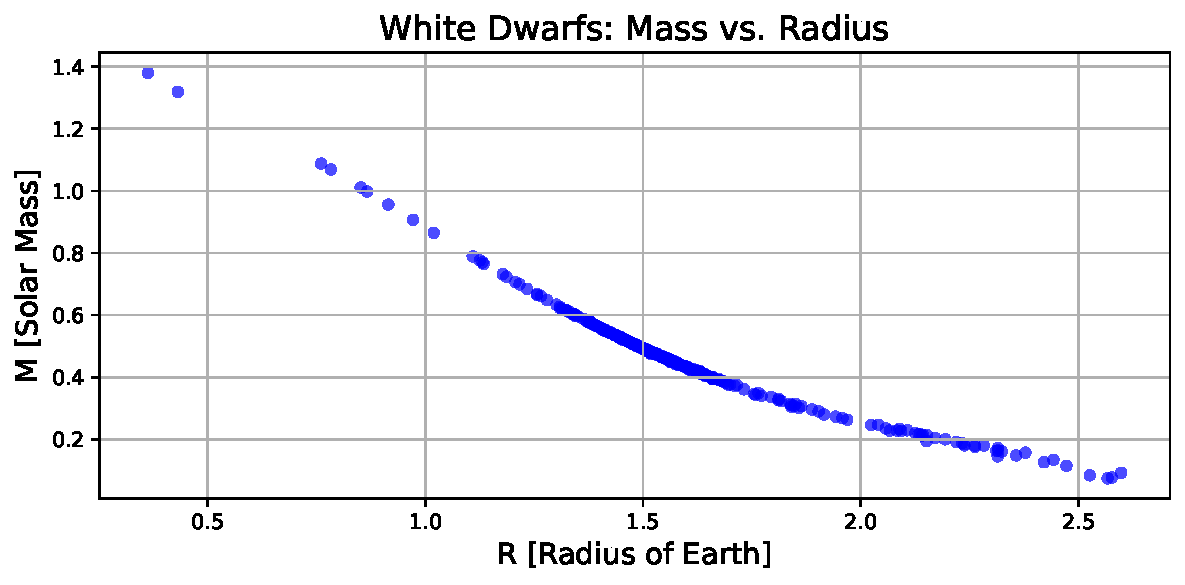
\includegraphics[width=0.8\textwidth]{Newton_PartB_WhiteDwarfDataFitting.pdf}
    \caption{Visualization of the white dwarf data.}
    \label{fig:newton-partb}
\end{figure}

\clearpage % Ensures the content after this starts on a new page

\section{Polytropic Fit for White Dwarfs}

We have the EOS for cold WDs (in CGS units for pressure):
\[
\boxed{
P(\rho)
~\,=\,~
C\,\Bigl[x\,(2x^{2}-3)\,\sqrt{1 + x^{2}} \;+\; 3\,\sinh^{-1}(x)\Bigr],
\quad
x \;=\;\Bigl(\tfrac{\rho}{D}\Bigr)^{\!\!1/q}.
}
\]
We want the leading term for \textbf{small} \(x\). This corresponds to \textbf{low-mass} WDs where the density \(\rho\) is still well below the scale set by \(D\).

\subsection{Series Expansion for Small \(x\)}

Let’s expand, term by term, for \(x \to 0\).

\subsubsection{Inside the Bracket \(\bigl[\ldots\bigr]\):}

\[
\begin{aligned}
x\,(2\,x^2 - 3)\,\sqrt{1 + x^2}
&=~
x\,\bigl(-3 + 2\,x^2\bigr)
\Bigl[\,1 + \tfrac{x^2}{2} - \tfrac{x^4}{8} + \dots\Bigr] 
\\[4pt]
&=
x\,\Bigl[-3 + 2x^2 + \dots\Bigr]
\Bigl[\,1 + \tfrac{x^2}{2} + \dots\Bigr]
\\[4pt]
&=
-3\,x + 0.5\,x^3 + 1.375\,x^5 + \dots
\quad(\text{we keep up to }x^5\text{ terms}).
\end{aligned}
\]

\subsubsection{The Term \(3\,\sinh^{-1}(x)\):}

Recall for small \(x\),
\[
\sinh^{-1}(x) = x - x^3/6 + (3/40)\,x^5 + \dots.
\]
Multiplying by 3 yields:
\[
3\,\sinh^{-1}(x)
~\approx~
3\,x \;-\;\tfrac{1}{2}\,x^3 \;+\; 0.225\,x^5 + \dots
\]

\subsubsection{Summation:}

Combining the terms:
\[
\begin{aligned}
\bigl[x\,(2x^2-3)\,\sqrt{1+x^2}\bigr] 
\;+\; 3\,\sinh^{-1}(x)
&~=~
\underbrace{(-3x + 3x)}_{0}
\\[6pt]
&\quad+\; \underbrace{(0.5\,x^3 - 0.5\,x^3)}_{0}
\\[6pt]
&\quad+\; \underbrace{(1.375 + 0.225)\,x^5}_{1.6\,x^5}
\;+\;\dots
\end{aligned}
\]

Hence, the first \textbf{nonzero} term is:
\[
= \frac{8}{5}\,x^5 \;+\;\mathcal{O}(x^7).\footnote{This derivation is also done by symbolic calculations through \texttt{sympy} in \href{Newton.ipynb}{Newton.ipynb part C.1} through series expansion.}
\]

Therefore:
\[
P(\rho)
~\approx~
C\;\frac{8}{5}\,x^5
\quad\text{for }x\to0.
\]

\subsubsection{Rewrite \(x = \bigl(\tfrac{\rho}{D}\bigr)^{1/q}\):}

\[
P(\rho)
~\approx~
\frac{8C}{5}\,\Bigl(\frac{\rho}{D}\Bigr)^{\!\!\tfrac{5}{q}}
~=~
\underbrace{\Bigl[\frac{8C}{5}\,\frac{1}{D^{5/q}}\Bigr]}_{K_{\star}}\,
\rho^{\,\tfrac{5}{q}}
\]
Hence the polytropic index in the exponent:
\[
P ~\propto~ \rho^{5/q}
\]
Compare to a standard polytrope:
\[
P ~\propto~ \rho^{1 + \tfrac{1}{n_{\star}}}
\quad\Longrightarrow\quad
1 + \frac{1}{n_{\star}} ~=~ \frac{5}{\,q\,}
\]
Solve for \(n_{\star}\):
\[
\frac{1}{n_{\star}} = \frac{5}{q} - 1 
= \frac{5 - q}{\,q\,}
~\Longrightarrow~
n_{\star} = \frac{q}{\,5 - q\,}
\]
And the overall coefficient:
\[
K_{\star} 
~=~
\frac{8\,C}{\,5\,}\;\frac{1}{D^{5/q}}.
\]
Thus:
\[
\boxed{
n_{\star} 
~=~ \frac{q}{\,5 - q\,},
\quad
K_{\star}
~=~
\frac{8\,C}{\,5\,}\;D^{-\tfrac{5}{q}}
}
\]

These final relations are exactly what we wanted to show.

\subsection{Figure: Line Fitting to White Dwarf Data}

Below, the fitted line to the White Dwarf data can be seen. The plotting is done in \href{Newton.ipynb}{Newton.ipynb, part C.2}.

\begin{figure}[H] % Use [H] to force the figure to stay in place
    \centering
    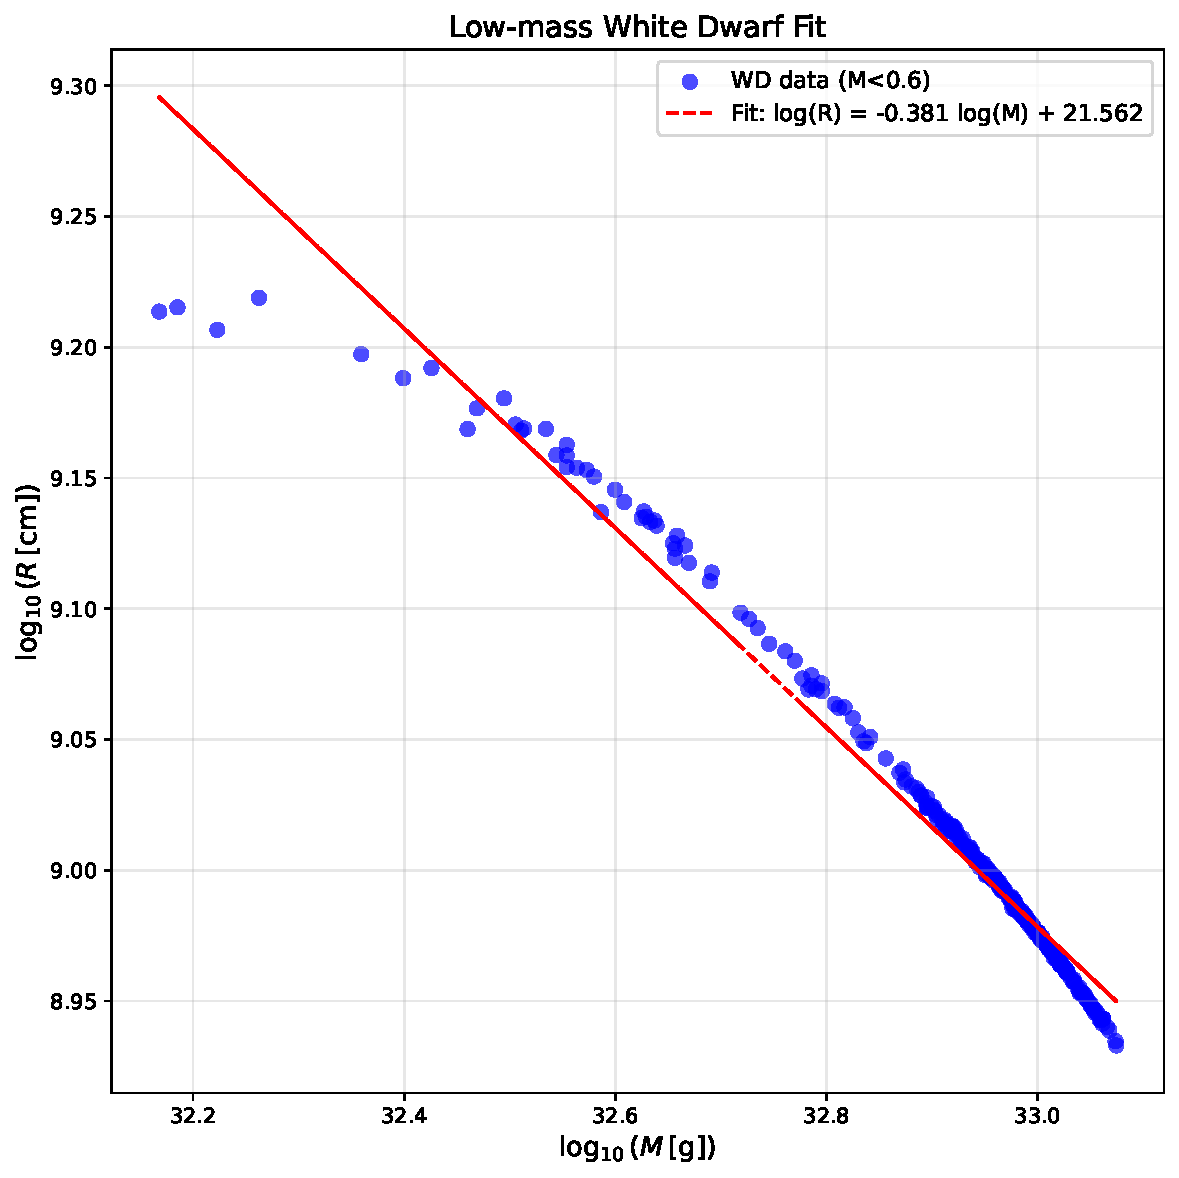
\includegraphics[width=0.8\textwidth]{Newton_PartC2.pdf}
    \caption{Fitting a line through the White Dwarf data.}
    \label{fig:newton-partc2}
\end{figure}

The results of the fitting process are as follows. The inferred polytropic index is \( n_\star = 1.5521 \). The effective scaling constant is given by
\[
c = 10^{\text{intercept}} = 3.6434 \times 10^{21} \, \mathrm{cm \, g^{-1/2}}.
\]
The effective constant \( K_\star \) was calculated using the scaling relation:
\[
K_\star = \frac{4 \pi G c^2}{(n_\star + 1)^2 \xi_1^2},
\]
where \( \xi_1 \) is the first zero of the Lane-Emden equation for \( n_\star = 1.55 \) (\( \xi_1 \approx 3.65 \)).

Finally, the calculated value of \( K_\star \) is:
\[
K_\star = 1.285 \times 10^{35} \, \mathrm{erg \, cm^{3(1-n_\star)} \, g^{-n_\star}}.
\]

\subsection{Figure: Central Density \(\rho_c\) vs Mass \(M\)}

The relationship between Central Density \(\rho_c\) and Mass \(M\) for White Dwarfs is shown below. The plots are generated in \href{Newton.ipynb}{Newton.ipynb, parts C.2.2 and C.2.3}.

\begin{figure}[H] % Use [H] to force the figure to stay in place
    \centering
    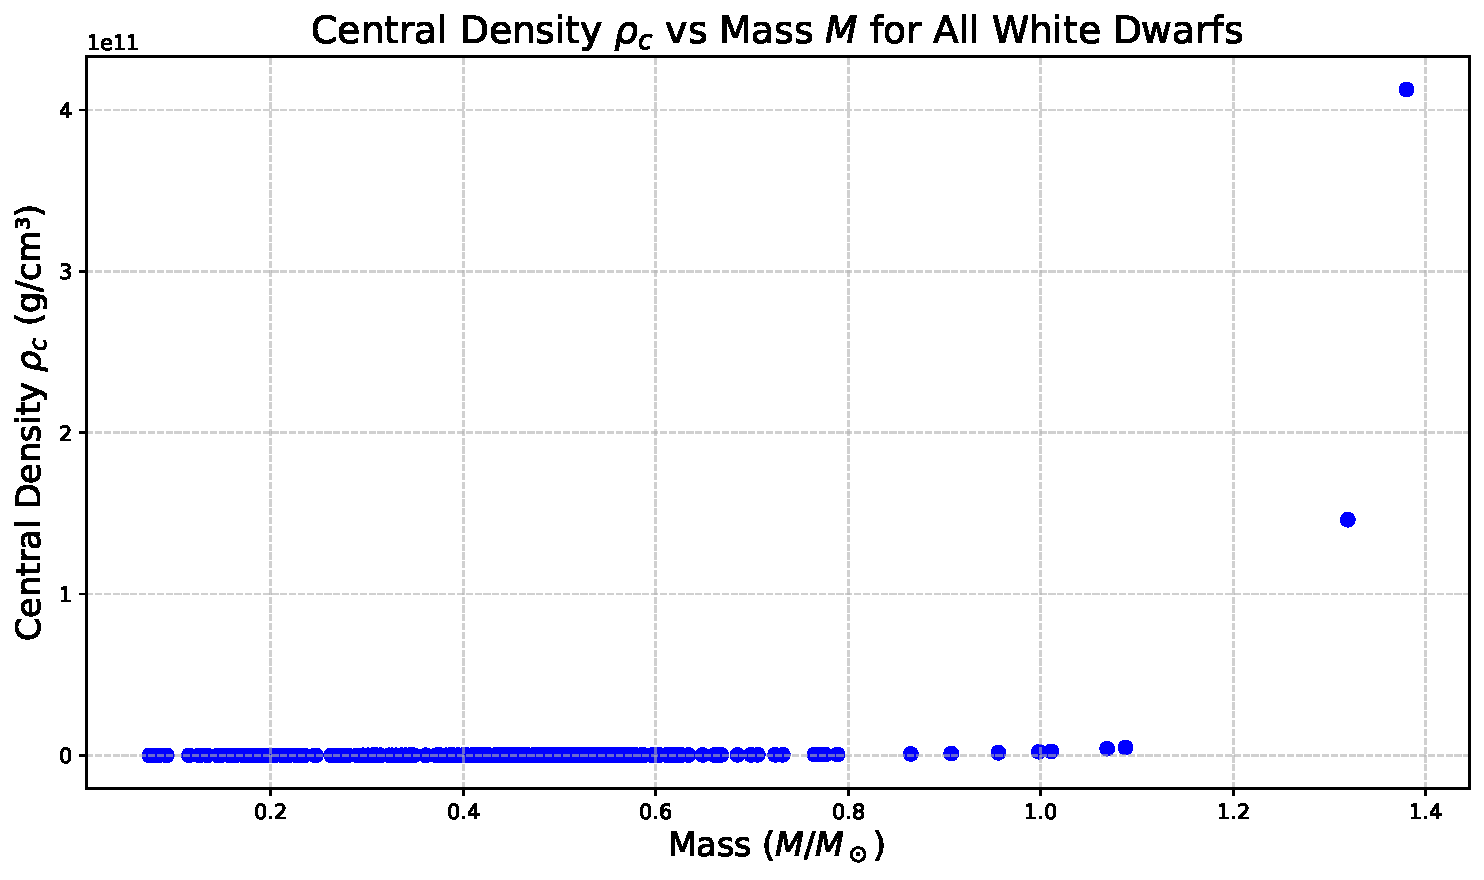
\includegraphics[width=0.8\textwidth]{Newton_PartC2.2.pdf}
    \caption{Plot of Central Density \(\rho_c\) vs Mass \(M\) for White Dwarfs. Full dataset shown to highlight the low-mass turning point.}
    \label{fig:newton-partc2.2}
\end{figure}

\begin{figure}[H] % Use [H] to force the figure to stay in place
    \centering
    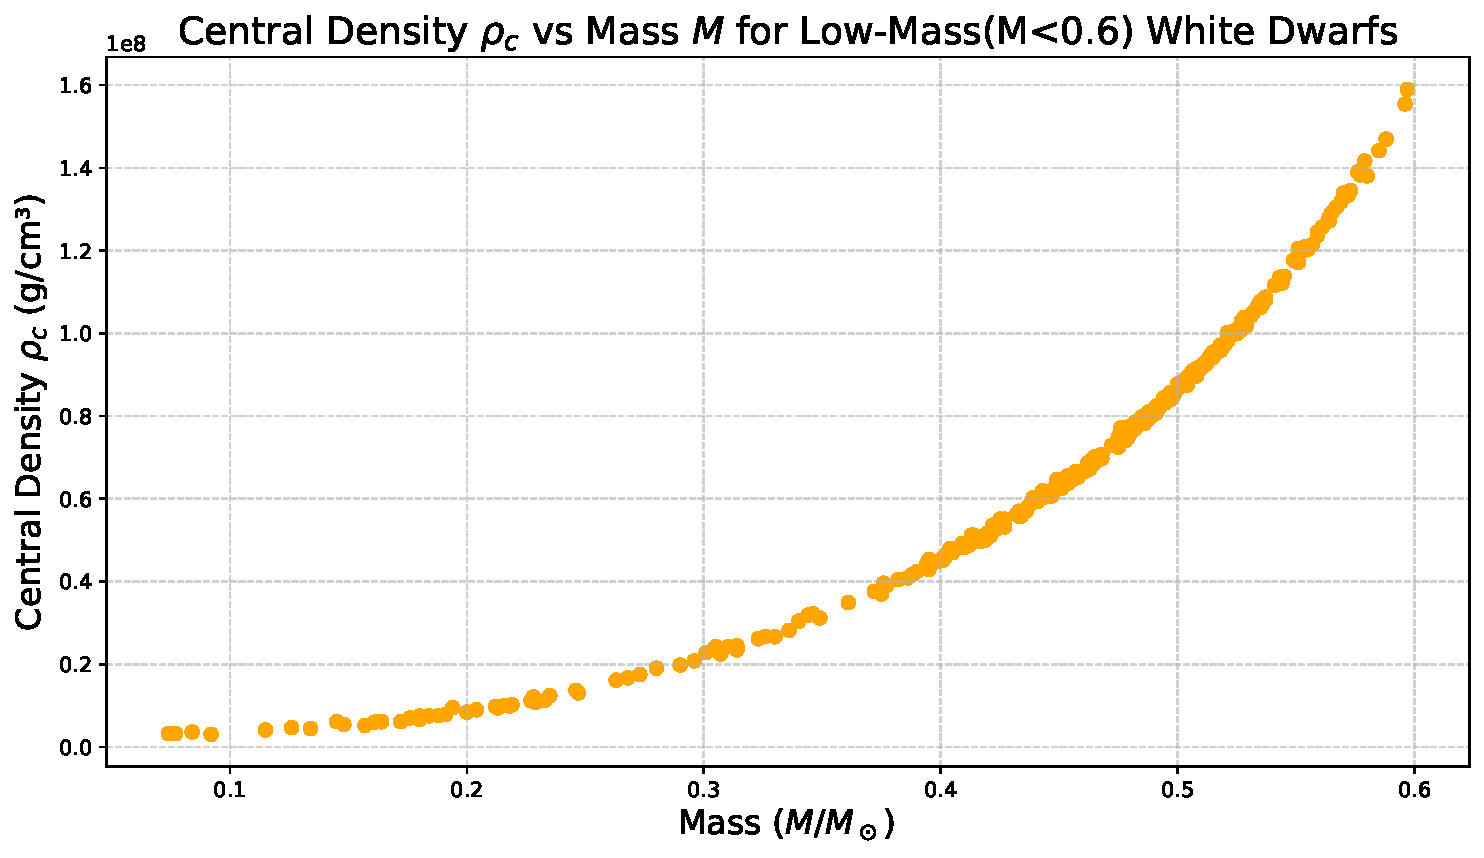
\includegraphics[width=0.8\textwidth]{Newton_PartC2.3.pdf}
    \caption{Focus on low-mass White Dwarf data.}
    \label{fig:newton-partc2.3}
\end{figure}

\clearpage

\section{Finding best fits of \(C\) and \(D\)}

\subsection{We Already Know \(q\)}

Previously, we assumed \(q \approx 3\). Substituting into the EOS for Cold WDs, we have:
\[
\boxed{
P(\rho)
\;=\;
C
\left[
  x\,\bigl(2x^2 - 3\bigr)\sqrt{x^2 + 1}
  \;+\; 3\,\sinh^{-1}(x)
\right],
\quad
x = \Bigl(\tfrac{\rho}{D}\Bigr)^{1/q}.
}
\]

Once \(D\) is chosen, we compute:
\[
C \;=\;\frac{5}{8}\;K_\star\;\bigl[D^{5/q}\bigr]
\quad\Longrightarrow\quad
\text{(thus, \(P(\rho)\) is fully specified).}
\]

\subsection{Hydrostatic Equilibrium IVP}

We solve the usual ODEs (in CGS units):
\[
\begin{cases}
\dfrac{dP}{dr} = -\,\rho(r)\,\dfrac{G\,m(r)}{r^2},\\[6pt]
\dfrac{dm}{dr} = 4\pi\,r^2\,\rho(r),
\end{cases}
\]
starting from \(r=0\) with
\[
\rho(0) = \rho_c,\quad
m(0) = 0.
\]

We integrate outward until \(\rho \approx 0\) (the star’s surface). At each step:
\[
P(r) = P(\rho(r)) \;=\; \text{(EOS for Cold WDs)},
\]
and invert \(P \leftrightarrow \rho\) numerically. Since we have an explicit expression for \(P(\rho)\), we can invert \(\rho(P)\) either using a small root-finding method inside the ODE solver or through a direct formula if the equation is rearranged appropriately. Alternatively, \(\rho\) can be kept as the integration variable, and \(d\rho/dr\) can be derived from \(dP/d\rho\).

\subsection{Getting \((R, M)\)}

Once \(\rho\) becomes negligible, we record:
\[
R_{\star}(\rho_c),\quad M_{\star}(\rho_c).
\]

By scanning over different \(\rho_c\) values, we produce discrete points:
\[
\bigl\{(R_i, M_i)\bigr\}_{i=1}^{10}.
\]
This process is performed \textbf{once} for a single choice of \(D\).

\subsection{Final Result}

The actual values of \(C\) and \(D\), calculated theoretically, are as follows:
\[
C = \frac{m^4 e^5}{24\pi^2 \hbar^3} = 6.002332185660436 \times 10^{21},
\]
\[
D = \frac{\mu m^3 e^3 \mu_e}{3\pi^2 \hbar^3} = 1.947864333345182 \times 10^{9}.
\]

Through computations from \href{Newton.ipynb}{Newton.ipynb, part D}, best-fitted values are as follows:
\[
\hat{D} = 3.3333 \times 10^{-6},
\]
\[
\hat{C} = 1.6938 \times 10^{12}.
\]

\clearpage

\section{Plotting the Full \(R\) vs \(M\) Curve}

\subsection{Full Electron-Degenerate EOS in the Relativistic Limit}

We start with the general $(T=0)$ electron degeneracy pressure:
\[
P(\rho) \;=\; C 
\Bigl[
  x\,(2x^2 - 3)\,\sqrt{1 + x^2}
  \;+\;
  3\,\sinh^{-1}(x)
\Bigr],
\quad
x \;=\;
\Bigl(\tfrac{\rho}{D}\Bigr)^{1/q},
\quad
\text{with }q = 3.
\]

\paragraph{Nonrelativistic limit ($x \ll 1$).}
By following part C.1.4 and substituting $q = 3$, one finds $P \propto \rho^{5/3}$, i.e.\ a polytrope with $n=\tfrac{3}{2}$ .

\paragraph{Ultrarelativistic limit ($x \gg 1$).}
Expanding the expression in the $P(\rho)$:
\[
x\,(2x^2 -3)\,\sqrt{1 + x^2} \;+\; 3\,\sinh^{-1}(x)
\]
for $x\to\infty$ using symoblic computations from \href{Newton.ipynb}{Newton.ipynb, part E.1}: gives a leading term \emph{proportional to} $x^4$:
\[
x\,(2x^2 - 3)\,\sqrt{1 + x^2}
\;\approx\;
2\,x^4
\quad
\text{as }x\to\infty,
\]

After substituting $x^3 = \rho/D$, we get: 
\[
P(\rho)\;\propto\;\rho^{4/3},
\]
which corresponds to a polytrope of index $n=3.$

Thus, the \textbf{relativistic limit} yields $P(\rho)\propto \rho^{4/3}$, and $n=3$.  

\subsection{Chandrasekhar Mass via \(n=3\) Polytrope}

From polytrope theory (Lane–Emden approach), the mass-radius relation for a polytrope of index \(n\) is summarized as:
\[
M \;\propto\; R^{\,\frac{3 - n}{\,1 - n\,}}.
\]
For \(n < 3\), this results in a continuous family of solutions. However, when \(n=3\), the exponent becomes:
\[
\frac{3 - 3}{1 - 3} \;=\; 0,
\]
which means \(M\) becomes a \textbf{constant}, independent of \(R\). Physically, this implies the star’s mass saturates at a maximum value in the ultrarelativistic regime, known as the \textbf{Chandrasekhar mass}, \(M_{\mathrm{Ch}}\).

\subsubsection{Analytical Formula}

From detailed polytrope analysis, the Chandrasekhar mass is given (in CGS units, for \(\mu_e=2\)) by:
\[
M_{\mathrm{Ch}}
\;=\;
\underbrace{\kappa}_{\text{a constant of nature}}
\;\bigl(\mu_e\bigr)^{-2}\,,
\]
where \(\kappa\) depends on \(\hbar\), \(c\), \(m_e\), etc. Substituting:
\[
C \;=\; \frac{m_e^{4}\,c^{5}}{24\pi^{2}\,\hbar^{3}},
\quad
D \;=\; \frac{m_u\,m_e^{3}\,c^{3}\,\mu_e}{3\pi^2\,\hbar^3},
\quad
\mu_e=2,
\]
and performing the polytrope calculations for \(n=3\), we recover the well-known result:
\[
M_{\mathrm{Ch}}
\;\approx\;
1.44\,M_{\odot}
\]

\subsection{Numerical Confirmation}

When solving the full EOS over a range of central densities \(\rho_c\), the White Dwarf mass \(M(\rho_c)\) initially increases with \(\rho_c\) but eventually peaks and begins to \textbf{decrease} for very high \(\rho_c\). This peak corresponds to the Chandrasekhar limit, beyond which no stable solutions exist.

\subsection{Figure: Full Mass-Radius Curve}

The full mass-radius curve for White Dwarfs is shown below. The plotting is done in \href{Newton.ipynb}{Newton.ipynb, part E.2}.
\begin{figure}[H] % Use [H] to force the figure to stay in place
    \centering
    \includegraphics[width=0.8\textwidth]{Newton_PartE2_theorotical.pdf}
    \caption{Full mass-radius curve for White Dwarfs using theorotical \(C\) and \(D\) values.}
    \label{fig:newton-parte2t}
\end{figure}

\begin{figure}[H] % Use [H] to force the figure to stay in place
    \centering
    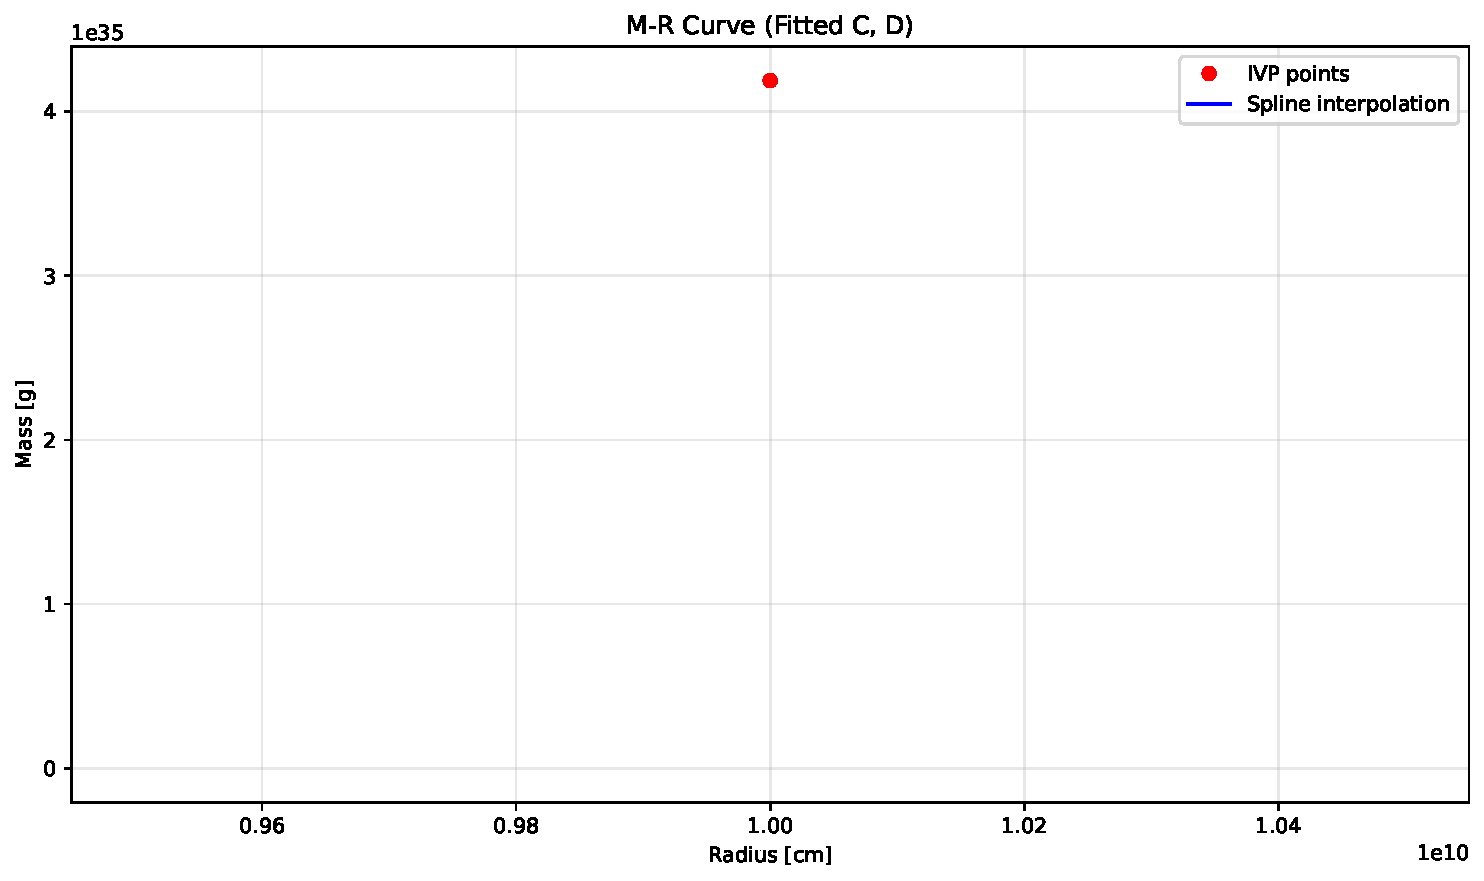
\includegraphics[width=0.8\textwidth]{Newton_PartE2_calculated.pdf}
    \caption{Full mass-radius curve for White Dwarfs using fitted \(C\) and \(D\)values.}
    \label{fig:newton-parte2c}
\end{figure}

\end{document}